\documentclass[tikz, border=2pt]{standalone}

\usepackage{amsmath,amssymb}
\usepackage{pgfplots}
\pgfplotsset{compat=1.18}
\usepgfplotslibrary{groupplots}
\usetikzlibrary{arrows.meta}
\usepackage{xcolor}

\definecolor{utnblue}{RGB}{0, 51, 102}
\definecolor{utnred}{RGB}{204, 0, 0}
\definecolor{utngreen}{RGB}{0, 130, 70}

\begin{document}
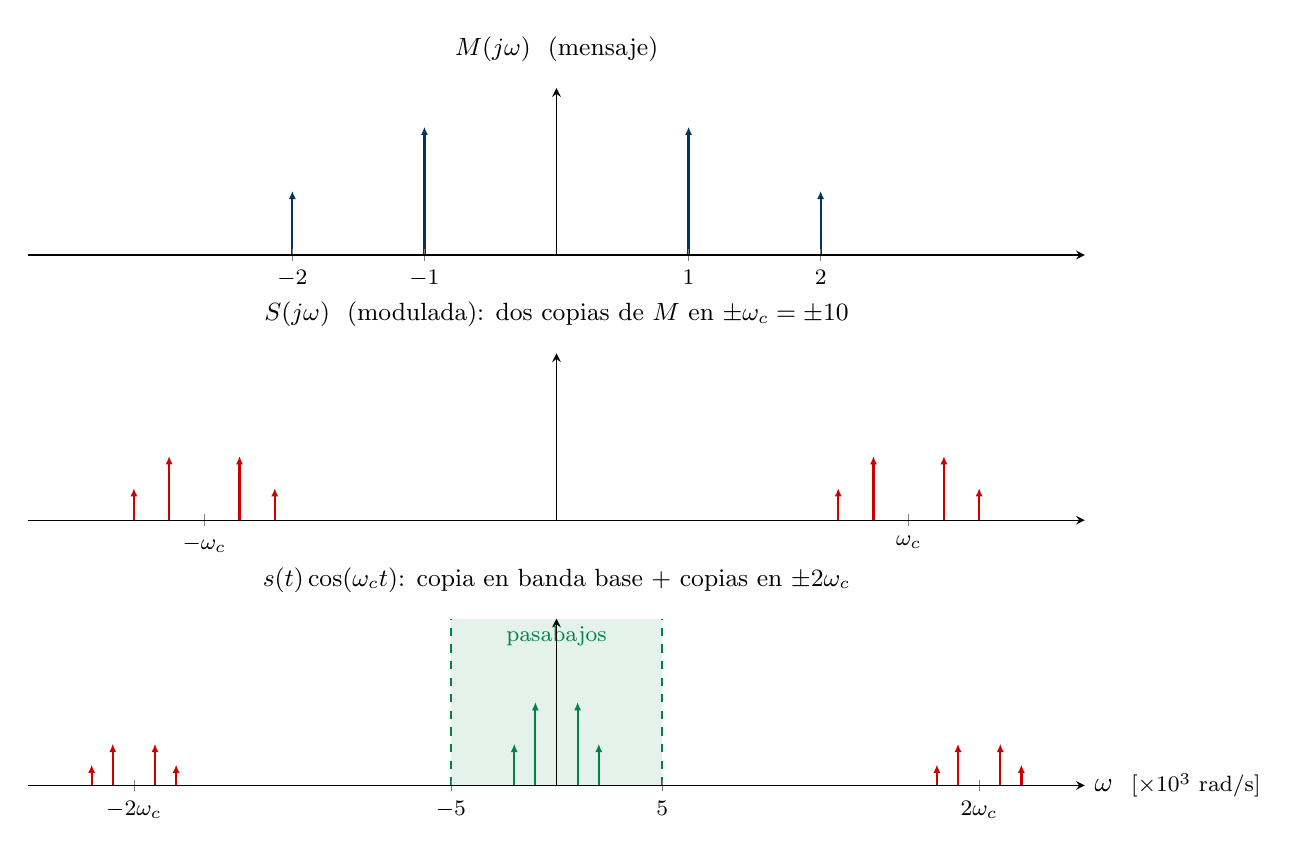
\begin{tikzpicture}[
    impb/.style={utnblue,  line width=0.8pt, -{Latex[length=3pt,width=2.6pt]}},
    impr/.style={utnred,   line width=0.8pt, -{Latex[length=3pt,width=2.6pt]}},
    impg/.style={utngreen, line width=0.8pt, -{Latex[length=3pt,width=2.6pt]}},
  ]

\begin{groupplot}[
    group style={group size=1 by 3, vertical sep=1.25cm},
    width=15cm, height=3.7cm,
    axis lines=middle,
    axis on top=true,
    enlargelimits=false,
    tick label style={font=\footnotesize},
    label style={font=\small},
    title style={font=\small},
    every axis x label/.style={at={(ticklabel* cs:1)}, anchor=west},
]

% --- Panel 1: M(jw) ---
\nextgroupplot[
    title={$M(j\omega)$ \ (mensaje)},
    xmin=-4, xmax=4, ymin=0, ymax=1.3,
    xtick={-2,-1,1,2}, xticklabels={$-2$,$-1$,$1$,$2$},
    ytick=\empty,
]
\draw[impb] (axis cs:-1,0) -- (axis cs:-1,1);
\draw[impb] (axis cs: 1,0) -- (axis cs: 1,1);
\draw[impb] (axis cs:-2,0) -- (axis cs:-2,0.5);
\draw[impb] (axis cs: 2,0) -- (axis cs: 2,0.5);

% --- Panel 2: S(jw) ---
\nextgroupplot[
    title={$S(j\omega)$ \ (modulada): dos copias de $M$ en $\pm\omega_c=\pm 10$},
    xmin=-15, xmax=15, ymin=0, ymax=1.3,
    xtick={-10,10}, xticklabels={$-\omega_c$,$\omega_c$},
    ytick=\empty,
]
\draw[impr] (axis cs:-12,0) -- (axis cs:-12,0.25);
\draw[impr] (axis cs:-11,0) -- (axis cs:-11,0.5);
\draw[impr] (axis cs: -9,0) -- (axis cs: -9,0.5);
\draw[impr] (axis cs: -8,0) -- (axis cs: -8,0.25);
\draw[impr] (axis cs:  8,0) -- (axis cs:  8,0.25);
\draw[impr] (axis cs:  9,0) -- (axis cs:  9,0.5);
\draw[impr] (axis cs: 11,0) -- (axis cs: 11,0.5);
\draw[impr] (axis cs: 12,0) -- (axis cs: 12,0.25);

% --- Panel 3: producto de demodulacion ---
\nextgroupplot[
    title={$s(t)\cos(\omega_c t)$: copia en banda base $+$ copias en $\pm 2\omega_c$},
    xlabel={$\omega$ \ \footnotesize[$\times 10^3$ rad/s]},
    xmin=-25, xmax=25, ymin=0, ymax=1.0,
    xtick={-20,-5,5,20}, xticklabels={$-2\omega_c$,$-5$,$5$,$2\omega_c$},
    ytick=\empty,
]
% banda de paso del filtro
\fill[utngreen!10] (axis cs:-5,0) rectangle (axis cs:5,1.0);
\draw[utngreen, dashed, thick] (axis cs:-5,0) -- (axis cs:-5,1.0);
\draw[utngreen, dashed, thick] (axis cs: 5,0) -- (axis cs: 5,1.0);
\node[font=\footnotesize, utngreen, anchor=south] at (axis cs:0,0.78) {pasabajos};
% banda base recuperada (1/2 m)
\draw[impg] (axis cs:-1,0) -- (axis cs:-1,0.5);
\draw[impg] (axis cs: 1,0) -- (axis cs: 1,0.5);
\draw[impg] (axis cs:-2,0) -- (axis cs:-2,0.25);
\draw[impg] (axis cs: 2,0) -- (axis cs: 2,0.25);
% copias en +/- 2wc
\draw[impr] (axis cs:-22,0) -- (axis cs:-22,0.125);
\draw[impr] (axis cs:-21,0) -- (axis cs:-21,0.25);
\draw[impr] (axis cs:-19,0) -- (axis cs:-19,0.25);
\draw[impr] (axis cs:-18,0) -- (axis cs:-18,0.125);
\draw[impr] (axis cs: 18,0) -- (axis cs: 18,0.125);
\draw[impr] (axis cs: 19,0) -- (axis cs: 19,0.25);
\draw[impr] (axis cs: 21,0) -- (axis cs: 21,0.25);
\draw[impr] (axis cs: 22,0) -- (axis cs: 22,0.125);

\end{groupplot}

\end{tikzpicture}
\end{document}
